%!TeX root=../tese.tex
%("dica" para o editor de texto: este arquivo é parte de um documento maior)
% para saber mais: https://tex.stackexchange.com/q/78101


\chapter{Models}
\label{chap:models}

In this chapter we will be exploring the different components of the models we developed and the motivation behind our decisions. Lastly the hyper-parameters choice and the optimization of the different models trained  will also be briefly explored. 



\section{Embeddings}

To create our function extraction models we need to be able to calculate an embedding for code functions. However, none of the previously explored code embeddings in Chapter~\ref{chap:related_work} are granular enough for our needs, they expect whole functions while we need to be able to at the very least create embeddings per line of code. Exploring the literature, in particular \citet{allamanis2018survey} which presents a table of over 30 code embedding generators for a diverse range of tasks, we were not able to find a fitting embedding. One of our original objectives was to develop our own code embedding for this task, however due to time constraints caused by the dataset delay this was no longer feasible.



So, once again leveraging the idea of naturalness of programming languages that we introduced in Chapter~\ref{chap:intro} we opted to utilize embeddings for natural languages --- in particular english --- to represent our code.


There were two main types of embeddings tested in this project: the more traditional GloVe based embeddings and the transformer based embeddings that we had the opportunity of exploring during the semester abroad at TUDelft thanks to the FAPESP BEPE program. Both embeddings are sentence embeddings, i.e. each line of code will have its own vector embedding. Here we will give a short  overview of how these embeddings work and how they were built.



\subsubsection{Transformer based}


Following our initial goal of exploring the use of transformers for refactoring tasks we arrived at two main approaches: utilizing transformers in our embedding and/or as our model. However, due to our time constraints imposed by our need to create our dataset from scratch, we focused on utilizing transformer based embeddings as the first step since adapting the dataset to be compatible with training a transformer model would be an extremely manual and time consuming process. Another relevant point is the maxim of ``garbage in garbage out'', that essentially states that if your data is bad your results will also be bad. We concluded that it would be more beneficial to first make sure that we have at least one reasonable embedding for our code before we start investing such a huge amount of our scarce time in adopting this new architecture. Unfortunately, by the time we finished exploring the use of transformer based embeddings, there was no feasible way of training a transformer model in the remaining time of the BEPE project. Therefore, in this section we will be exploring the use of transformer based embeddings and their performance compared to more traditional embeddings.


Among the many embedding options available for our analysis we chose to utilize the transformer based models of the SBERT project \citep{sbert_paper}. Until recently this project was referred to as the state of the art in many tasks involving sentence embeddings, furthermore it possesses embeddings trained through a diverse number of transformer based architectures with most of them being more computationally efficient when compared to other models such as BERT \citep{BERT} or RoBERTa \citep{roberta}.



In Fig.~\ref{embeddings}, also available as an interactive table at \citet{link_sbert_tabela}, we can see the main 13 models of interest available in the SBERT project and some metrics regarding them. Due to our time constraints we were forced to select only a few of these embeddings for our experiment, since they may take an entire day to train a single epoch. From this list we discarded all models solely trained on Q\&A datasets since they are too distinct from our real objective and other models that were too derivative of another model already present in the list such as \textit{all-MiniLM-L6-v2} (half the layers of \textit{all-MiniLM-L12-v2}), \textit{distiluse-base-multilingual-cased-v2} (trained in an additional 35 languages in comparison to \textit{distiluse-base-multilingual-cased-v1} but since most of our Java files are believed to be written in english we don't believe this would bring us significant gains in performance) and \textit{paraphrase-multilingual-mpnet-base-v2} (a slow and more inefficient version of \textit{all-mpnet-base-v2} that was trained in a smaller and more specific dataset). 


\begin{figure}[!ht]
\centerline{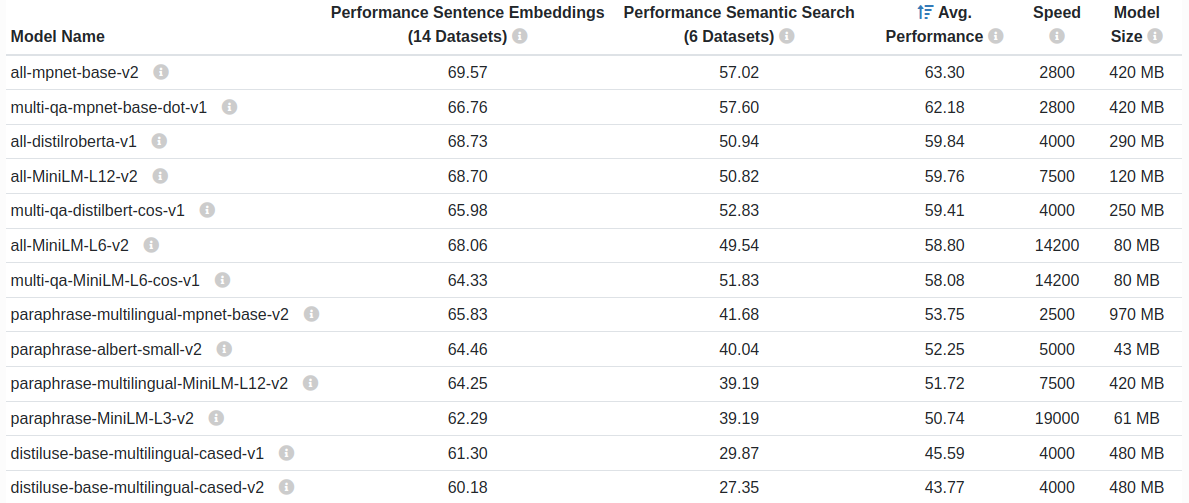
\includegraphics[scale=0.62]{embeddings.png}   }
\caption{Table of 13 embedding models available in the SBERT project and some metrics regarding them. \citep{link_sbert_tabela}}
\label{embeddings}
\end{figure}


After short-listing the available embeddings we were left with 7 embeddings to test out:
\begin{itemize}
    \item all-mpnet-base-v2 \citep{mpnet} \href{https://huggingface.co/sentence-transformers/all-mpnet-base-v2}{(Model Card)}
    \item all-distilroberta-v1 \citep{roberta, distillbert} \href{https://huggingface.co/sentence-transformers/all-distilroberta-v1}{(Model Card)}
    \item all-MiniLM-L12-v2 \citep{minilm}  \href{https://huggingface.co/sentence-transformers/all-MiniLM-L12-v2}{(Model Card)}
    \item paraphrase-albert-small-v2 \citep{albert}  \href{https://huggingface.co/sentence-transformers/paraphrase-albert-small-v2}{(Model Card)}
    \item paraphrase-multilingual-MiniLM-L12-v2 \citep{minilm}  \href{https://huggingface.co/sentence-transformers/paraphrase-multilingual-MiniLM-L12-v2}{(Model Card)}
    \item paraphrase-MiniLM-L3-v2 \citep{minilm}  \href{https://huggingface.co/sentence-transformers/paraphrase-MiniLM-L3-v2}{(Model Card)}
    \item distiluse-base-multilingual-cased-v1 \citep{distillbert}  \href{https://huggingface.co/sentence-transformers/distiluse-base-multilingual-cased-v1}{(Model Card)}
\end{itemize}


\subsubsection{GloVe}

GloVe \citep{glove} is a more traditional model that combines the advantages of two model families, local context windows and global matrix factorization. 
The model produces a vector space with meaningful sub-structure by leveraging statistical information in an efficient manner when training only on the nonzero elements in a word-word co-occurrence matrix, rather than on individual context windows in a large corpus or on the entire sparse matrix. 

At the time this method was published it attained state-of-the-art performance on the word analogy task, and outperformed other methods (such as word2vec) on several word similarity tasks.



By utilizing GloVe we also have an interesting counter-point to our transformer based embedding, we are essentially comparing an older and well established model that is still relevant even in this ever evolving field (the same cannot be said about bag-of-words for example) to what is essentially the more recent and generally successful approach.


By taking the average of the word embeddings of a sentence it is possible to generate an embedding for that sentence. This is what was done by \citet{sbert_site} in order to generate two GloVe sentence embedding models, one trained with 6 billion parameters and the other with 840 billion parameters.





\section{Architecture}

An important issue to be addressed here comes from a fundamental difference between natural languages and programming languages: even if a sentence in english has a grammatical mistake it is capable of transmitting meaning, of carrying a semantic value. The same cannot be said about a grammatically incorrect piece of code.
For this reason we are not able to blindly apply seq2seq NLP models on source code, we need to ensure that the code transformations we generate will not grammatically break the inputted code. To ensure the grammatical correctness of our refactoring we briefly explored the possibility of using language servers to intermediate our operations in Section~\ref{sec:lsp}.


Given this, our models simply needs to predict the line number of the start and end of the extracted linespan.


\begin{figure}[!ht]
\centering
\centerline{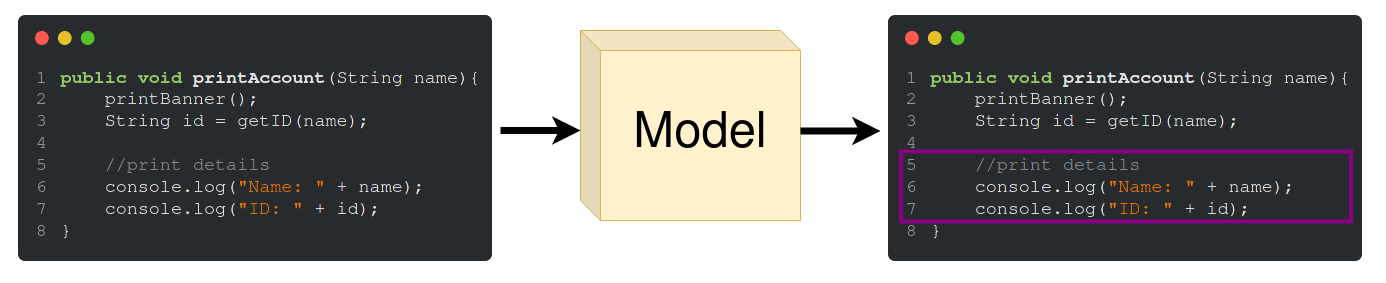
\includegraphics[scale=0.35]{figuras/modelo.png}}
\caption{Our model will receive the source code of a function definition that needs to be refactored and will output the line span that needs to be extracted. In this particular example the lines 5 to 7 of the \texttt{printAccount()} function need to be extracted.}
\label{modelo}
\end{figure}

\begin{figure}[!ht]
\centering
\centerline{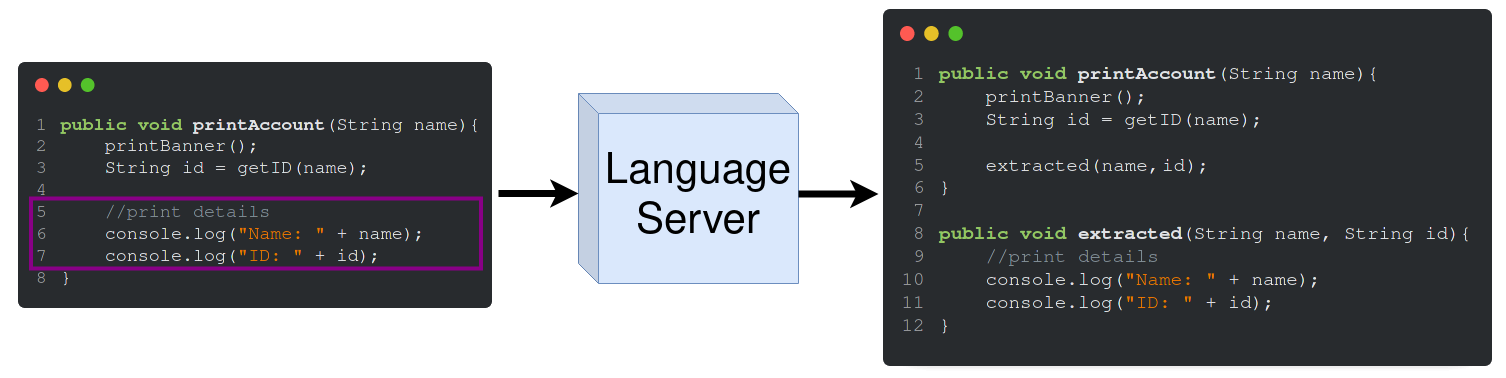
\includegraphics[scale=0.33]{figuras/lsp_refac.png}}
\caption{Once the line span of the extraction has been determined, the language server is contacted and it will be responsible for realizing the extraction and returning the refactored code. In this example the lines 5 to 7 are refactored by the language server and become the function \texttt{extracted()}.}
\label{lsp_refac}
\end{figure}

 In short, the model will be fed with the lines of a function one by one and it will generate as an output 2 pointers, one indicating the first line to be extracted and a second pointer indicating the last line to be extracted. Together these 2 pointers will define the line span to be refactored. Fig~\ref{modelo} presents a general illustration of our models, working as a black box, and Fig~\ref{lsp_refac} illustrates the refactoring done through a language server with the output of the black box model from Fig.~\ref{modelo}.



\subsubsection{Simple RNN}

Our first architecture is extremely simple; it consists of a LSTM layer that receives the embedded inputs and then passes on its hidden state to two different feedforward linear layers which will predict the start and end lines of the function extraction. 
As for the loss we chose the L1 distance function.



\subsubsection{Pointer Network (Ptr-Net)}

 Pointer Networks \citep{pointer} are a flexible encoder decoder model that utilizes attention to select one of the inputs as an output at each decoding step. As mentioned in Section~\ref{sec:ptrnet}, this model has been used in a variety of tasks that involve re-ordering and/or selecting elements of the inputted data. This is particularly useful in our case since our objective can be formulated as selecting which lines of an inputted function that need to be extracted, in particular at which line the extraction begins and ends. 

Our implementation of the pointer network utilizes a 1 layer LSTM as the encoder and another 1 layer LSTM as the decoder with the additive attention mechanism from \citet{bahdanau} tying them together. Lastly, to convert from the attention scores into the predicted lines we apply the softargmax function in order to apply the argmax function in a differentiable manner.



$$\textit{softargmax}(x)=\sum_i \frac{e^{\beta x_i}}{\sum_j e^{\beta x_j}}i$$

$\beta$ essentially controls how well this function approximate the argmax function, however a high enough $\beta$ will approximate it so well that back-propagation will start to fail. In Appendix~\ref{ap:beta} we present a brief exploration of the impact of $\beta$ on the model capability to learn. Luckily, our experiments did not detect any significant increase in performance by increasing $\beta$ over the value of 10, which is well below the point were back-propagation starts to fail.

We opted to use this function instead of the more commonly utilized softmax function in order to use the L1 loss instead of negative log likelihood loss. Since we are not predicting simple classes as our output, the error from missing the start of a refactoring by one line should be smaller than that of missing by 10 lines and this isn't possible with negative log likelihood. 
In Fig.~\ref{arquitetura} we can see an illustration of how this model works, particularly how the attention mechanism ``chooses'' the start and end of a function extraction. 





\begin{figure}[!ht]
\centerline{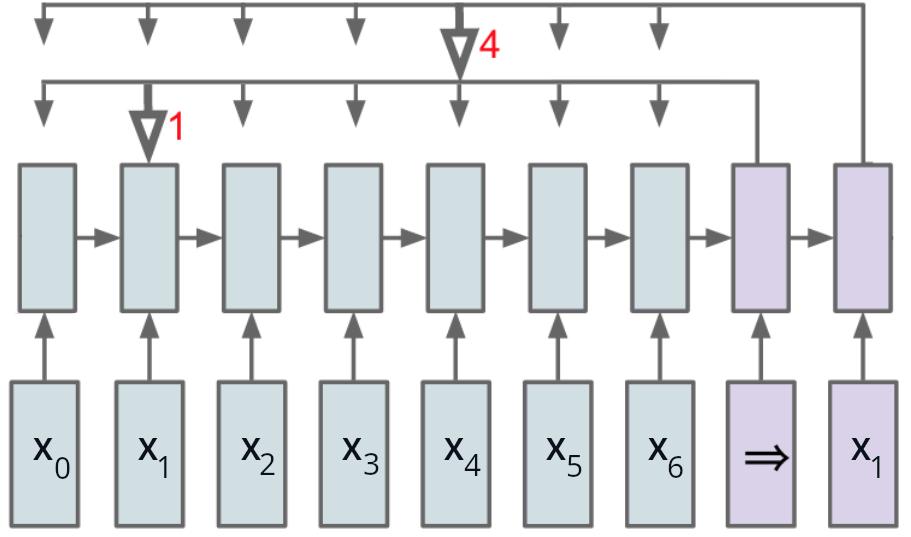
\includegraphics[scale=1.62]{arquitetura.png}   }
\caption{An illustration of how the model works, with green blocks representing the encoder and the purple ones the decoder. Each $x_i$ value fed to the encoder represents the embedding of a single line from the function being analyzed. The decoder receives as an input the hidden state from the last step (if available) and all the encoder hidden states, so to predict the last line to be extracted the decoder will receive all the hidden states from the encoder and the hidden state from last step that represents the first line to be extracted. Lastly, the attention mechanism is represented by the arrows pointing into the different encoder hidden states/inputs, the arrows may be seen as the final output of the model after the attention scores go through the softargmax function. So in this particular example being illustrated, the function is composed of 7 lines and it should go through an extraction of lines 1 through 4.}
\label{arquitetura}
\end{figure}




\section{Metrics}

When dealing with a well researched topic one is able to build upon previous knowledge and conventions in the area. However, to the best of our knowledge, there is no previous research that aims to automate the task of function extractions so we are faced with the challenge of defining how to best evaluate the quality of a predicted refactoring. In Section~\ref{sec:bleu} we explored a few common seq2seq metrics of NLP and their limitations, however none of the metrics presented are applicable for this particular use case, neither are the other metrics we could find in the literature. They may not be applicable to our particular use case but we may still take insights from them, such as BLEU's limitations that do not take into account if a sentence actually makes any semantic or grammatical sense. 

So without being able to resort to a readily available NLP metric we turned ourselves to typical code quality metrics, such as the ones presented in Section~\ref{sec:code_metrics}. Albeit these metrics can be useful in certain occasions we found them to be lacking for our needs. They can present a score of the code quality but by their very nature they are subjective since they try to give a concrete score to an abstract and subjective concept like code quality. Simply deciding which metric to use can bring vastly different results since not all of them are tailored towards the same issues and they do not operate on the same scales, comparing the pure score of different code metrics is akin to comparing apples to oranges.
Apart from that, our model performs only function extractions, the only code operation would be a transfer of code lines from an existing function to a newly created one, this would not bring a big impact in most code quality metrics. We could directly measure the size of functions instead of relying in more complicated code metrics but this would pose a new problem on itself, fewer lines of code does not necessarily equate to a better piece of code nor does a bigger extraction imply a better refactoring than a shorter one.
Besides, these metrics are not very actionable, they do not always present a clear path on how to improve the refactoring to maximize them.


Another early idea was to leverage unit tests to verify code integrity, however it is not guaranteed that all functions being refactored have unit tests nor that we would be able to easily identify them in a programmatic manner. Also, unless the linespan breaks a loop or some other flow control structure (which could be easily detected) the extraction would necessarily be a code preserving transformation so code integrity is not a concern.

Lastly we turned to classic ML metrics, such as accuracy.
We decided to utilize the binary accuracy, which is essentially equivalent to jaccard score, to measure how close the overlap between the predicted linespan and the ground truth is.

The jaccard coefficient is a measure of similarity between sets, defined as \citep{jaccard1912distribution}:
$$J(A,B) = \frac{|A \cap B|}{|A \cup B|} $$

An illustration of the jaccard index can be seen in Fig.~\ref{fig:jaccard_iou}.

\begin{figure}[!ht]
\centerline{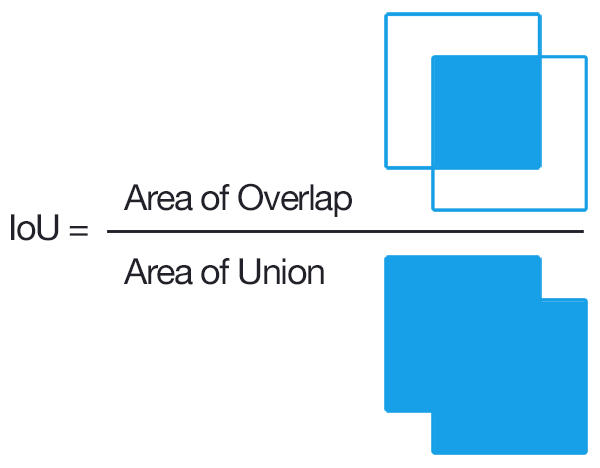
\includegraphics[scale=0.4]{figuras/iou.png}   }
\caption{A visual representation of the jaccard index. Image from \citet{iou}.}
\label{fig:jaccard_iou}
\end{figure}


Lastly, if an IDE plugin were to be implemented there would be the possibility of utilizing telemetry to evaluate user response to suggested refactorings. This would be a way to grasp the quality of suggested refactorings and to better understand when and why our model fails, however this is left for future work since such an endeavor was unfeasible given the time constraints of this project.


\section{Hyper-parameter choice}
\label{optuna}

Many scientific fields currently suffer from a reproducibility crisis \citep{reproducibility} and machine learning is no exception \citep{repro1, repro2, repro3, repro4}. So in the interest of transparency and reproducibility we include this section to explicitate how we arrived at our models hyper-parameters, i.e. the motivation and constraints behind our choices and the techniques used.


Originally we intended to optimize every single one of our models to the best of our ability in order to obtain the best performance possible, given our choices of architecture and embeddings. However due to time constraints this was simply not feasible, for instance training one epoch of some of the models that used transformer-based embeddings could take more than a whole day of training. That's why we had to compromise and decide exactly what was feasible to optimize and what would bring the greatest chance of improving the performance of our models.


We ended up deciding to optimize our pointer network models that utilized the GloVe based embeddings and when applicable to extrapolate our findings into the other models. More specifically we decided to optimize the following hyperparameters:


\begin{itemize}
\item Learning rate
\item Weight decay
\item Embedding
\item Batch size
\item Hidden size
\end{itemize}


To perform this optimization we split our dataset into training, validation and test and then we utilized the Optuna library from \citet{optuna} to optimize our model by training many trial runs on the training set and testing their performance in the validation set. 

\begin{figure}[!ht]
\centerline{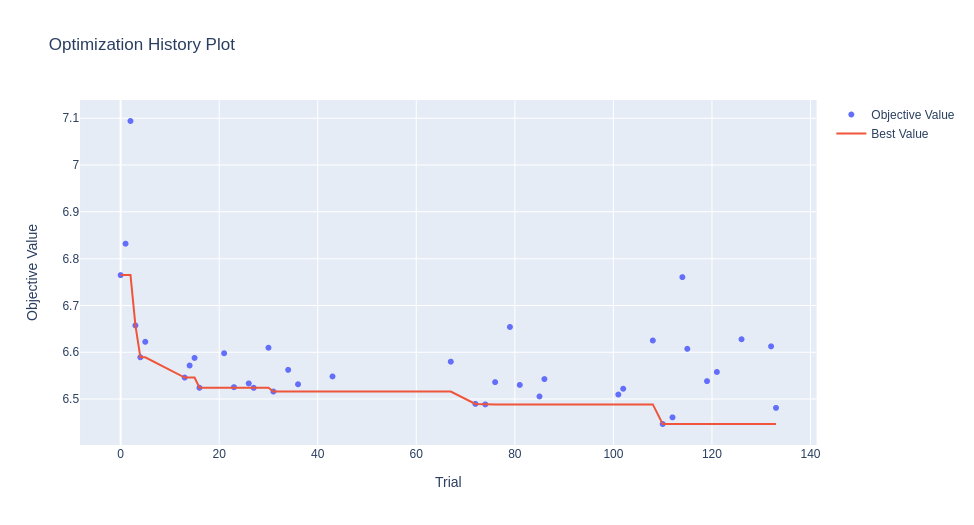
\includegraphics[scale=0.45]{opt_history.png}   }
\caption{Optimization history plot of the 136 Optuna trials.}
\label{hist}
\end{figure}


 After a warm-up period this library is capable of pruning any given run that is not achieving a satisfactory performance,  by doing this it is capable of exploring the parameter space in a more time efficient manner by only completing trial runs that have the possibility of achieving a better performance. 



There are many different samplers available in this toolbox, which essentially help us explore the parameter space by sampling different parameter values, and between all of them we chose to utilize the TPE (Tree-structured Parzen Estimator) \citep{tpe}.  
An important point of note about this sampler is that it assumes that the different hyperparameters are independent so it determines the value of a single parameter without considering any relationship between parameters. If this assumption is false the optimization  process may take more time or in some cases even miss some opportunities for further improvement when such hyperparameters have a strong relationship. We hypothesize that the hyperparameters that we chose are  independent or at the least have a weak impact on one another but since we have never tested this hypothesis it is possible that our model could be further optimized by simply picking a more robust sampler. Due to our time constraints we were unable to further explore this point.




Fig.~\ref{hist} presents the plot with the optimization history of our study and it's 196 trial runs and Fig.~\ref{optuna_all_runs} presents the loss and accuracy plots of these trials.

\begin{figure}[!ht]
\centerline{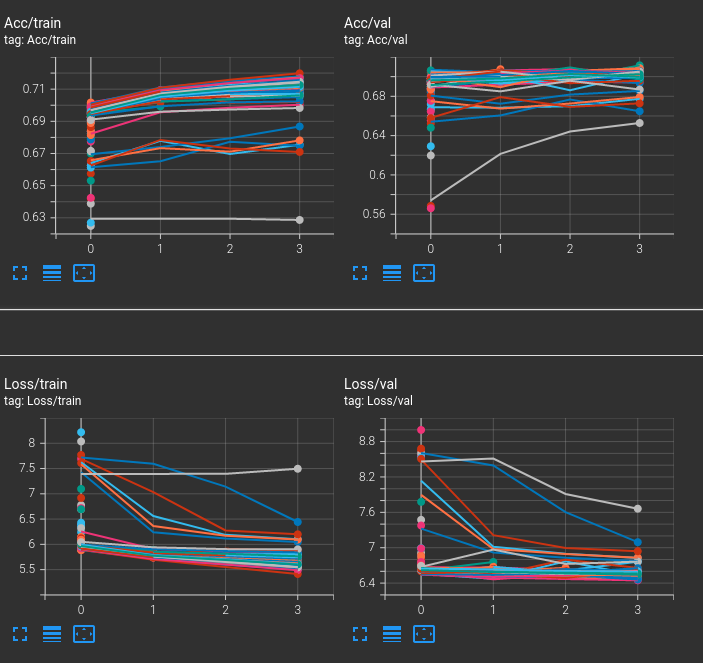
\includegraphics[scale=0.6]{figuras/optuna_all_glove_runs.png}   }
\caption{Loss and accuracy plots of the 196 Optuna trial runs.}
\label{optuna_all_runs}
\end{figure}


\begin{figure}[!ht]
\centerline{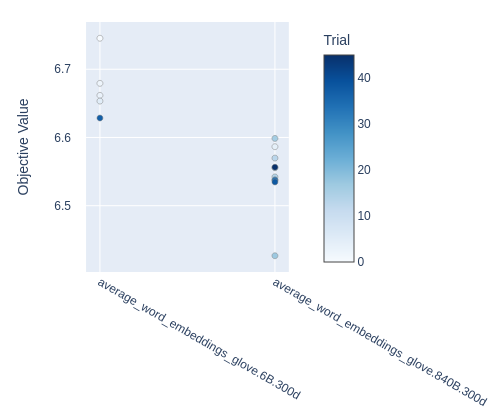
\includegraphics[scale=0.5]{slice glove editado.png}   }
 \caption{Slice plot of 43 Optuna trial runs, since the GloVe embedding trained with 840 billion parameters could achieve a better performance over it's counterpart trained with only 6 billion parameters we decided to exclude the embedding choice from the search space from our subsequent runs, as can be seen in Fig.~\ref{slice}.}
\label{sliceglove}
\end{figure}



\begin{figure}[!ht]
\centerline{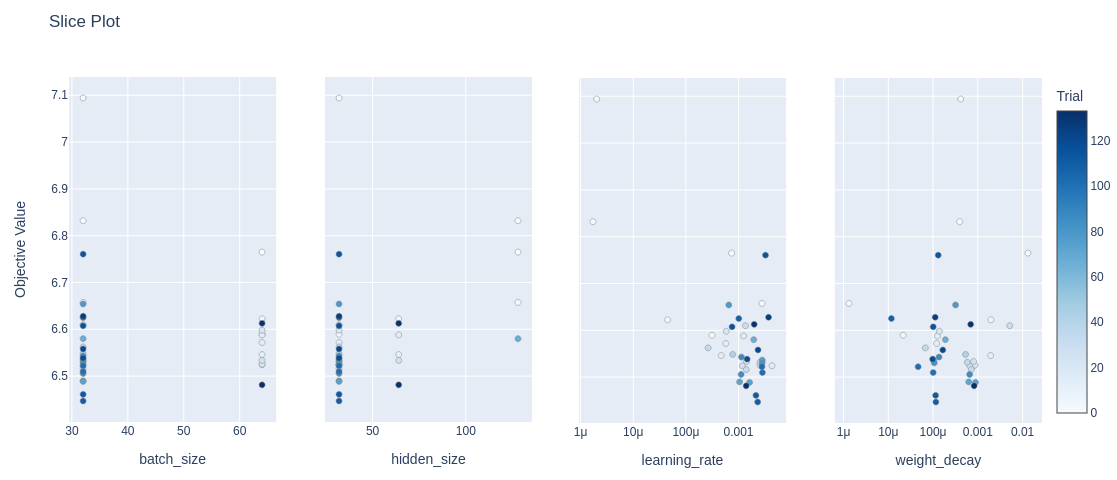
\includegraphics[scale=0.35]{slice2.png}   }
\caption{Slice plot of the optimization results found through Optuna. From the 136 trials, 95 were pruned before completion and 39 were completed. The best trial achieved a loss value of 6.446797407 with the following hyperparameter values:
    batch size= 32,
    hidden size= 32,    learning rate= 0.00231519996,
    weight decay= 0.0001155681898}
\label{slice}
\end{figure}


In Fig.~\ref{sliceglove} and Fig.~\ref{slice} we are able to see the slice plots of our parameters. Originally we were going to explore all parameters at the same time in a single study, but while we were still learning how to use Optuna it became clear that the GloVe embedding trained with 840 billion parameters could achieve a better performance over it's counterpart trained with only 6 billion parameters so we decided to exclude the embedding choice from the search space.









